\documentclass[hidelinks,a4paper,12pt, nofootinbib]{article}
\usepackage[nounderscore]{syntax}
\usepackage[left=3cm, top=2.5cm, right=2cm, left=2.5cm]{geometry}
\usepackage[spanish, es-tabla]{babel} %es-tabla es para que ponga Tabla en vez de Cuadro en el caption
\usepackage[utf8]{inputenc}
\usepackage[T1]{fontenc}
\usepackage{xspace}
\usepackage{xargs}
\usepackage{fancyhdr}
\usepackage{booktabs,tabularx}
\usepackage{multirow}
\usepackage{lastpage}
\usepackage{caratula}
\usepackage[bottom]{footmisc}
\usepackage{amsmath}
\usepackage{amssymb}
\usepackage{algorithm}
\usepackage[noend]{algpseudocode}
\usepackage{array}
\usepackage{xcolor,colortbl}
\usepackage{amsthm}
\usepackage{listings}
\usepackage{soul}
\usepackage[titletoc]{appendix}
\usepackage{pgf}
\usepackage{graphicx}
\usepackage{sidecap}
\usepackage{amsmath}
\usepackage{wrapfig}
\usepackage{caption}
\usepackage{subcaption}
\usepackage{tikz}
\usepackage{tikz-qtree}


%\usepackage{minted}

%Formato de los links
\usepackage{hyperref}
\hypersetup{
  colorlinks   = true, %Colours links instead of ugly boxes
  urlcolor     = blue, %Colour for external hyperlinks
  linkcolor    = blue, %Colour of internal links
  citecolor   = red %Colour of citations
}

\usepackage{comment}
%Bibliografia
\usepackage[
  backend=bibtex,
  style=alphabetic
]{biblatex}
\addbibresource{bibliografia.bib}


\captionsetup[table]{labelsep=space}


\setlength{\parindent}{4em}
\setlength{\parskip}{0.5em}


%%fancyhdr
\pagestyle{fancy}
\thispagestyle{fancy}
\addtolength{\headheight}{1pt}
\lhead{Aprendizaje Automático: TP1}
\rhead{$1º$ cuatrimestre de 2016}
\cfoot{\thepage\ / \pageref{LastPage}}
\renewcommand{\footrulewidth}{0.4pt}
\renewcommand{\labelitemi}{$\bullet$}
\setcounter{section}{-1}

%%caratula
\materia{Aprendizaje Automático}
\titulo{Trabajo Práctico Número 1}
%\subtitulo{}
%\grupo{Grupo COMPLETAR}
\integrante{Bordón, Pablo}{794/07}{bordonpablo@gmail.com}
\integrante{Gasco, Emilio}{171/12}{gascoe@gmail.com}
\integrante{Gatti, Mathias}{477/14}{mathigatti@gmail.com}

\fecha{28 de septiembre de 2016}

\usepackage{etoolbox}
\AtBeginEnvironment{tikzpicture}{\shorthandoff{>}\shorthandoff{<}}{}{}
\newcommand{\cupdot}{\mathbin{\mathaccent\cdot\cup}}
\title{AA}
\begin{document}
\maketitle

\tableofcontents
\newpage

\section{Extracción de atributos}

\begin{enumerate}

\item A continuación enumeramos los atributos que escogimos como potencialmente útiles y que luego implementamos para extraer automaticamente de los mails, estos fueron ideados por nosotros excepto por el atributo \textit{spell\_error\_count} el esta inspirado en el artículo \textit{Personalized Spam Filtering with
Natural Language Attributes}\footnote{https://pdfs.semanticscholar.org/8c64/21ad08277291813690c41c14a55916e46034.pdf}, en este paper se mencionan algunas buenas ideas mas las cuales no llegamos a implementar como contar la cantidad de palabras poco comunes o la cantidad de verbos en el texto.

\begin{itemize}
\item Los correos de spam suelen ser enviados a un único destinatario, para capturar esta característica se extraen 3 atributos del encabezado del correo: \textit{recipient\_count}, \textit{has\_cc} y \textit{has\_cc} para extraer cantidad de destinatarios del correo, si hay destinatarios en copia y si hay destinatarios en copia oculta respectivamente.
\item \textit{headers\_count} cantidad de encabezados.
\item \textit{mailer} Software utilizado para envió de correo. 
\item \textit{has\_body} Nos dice si el correo tiene cuerpo o si solo consta de encabezados
\item \textit{content\_type} Tipo del contenido del cuerpo de correo. Por ejemplo: text/plain, text/html, multipart/related, multipart/alternative,etc. 
\item \textit{content\_transfer\_encoding} la codificación utilizada para la transferencia del correo
\item \textit{is\_mulipart} Nos dice si el cuerpo consta de varias partes
\item \textit{subject\_length} Largo del título  del correo.
\item \textit{raw\_mail\_len} Largo del cuerpo del mensaje. 
\item \textit{raw\_body\_count\_spaces} Cantidad de espacios en cuerpo de correo.
\item \textit{has\_dollar} Nos dice si aparece el símbolo \$ en el cuerpo del correo. 
\item \textit{has\_link} Indica presencia de link http dentro del cuerpo del correo. 
\item \textit{has\_html} Indica presencia de html dentro del cuerpo del correo. 
\item \textit{has\_attachement} Indica la presencia de archivos adjuntos analizando content-type de las partes de correos con múltiples partes. Se consideran archivos adjuntos  a las partes que no sean del tipo text/*. 
\item \textit{uppercase\_count} Frecuencia de caracteres de letras mayúsculas en cuerpo de correo.  
\item \textit{has\_non\_english\_chars} Indica presencia de caracteres de idiomas diferentes al ingles dentro del cuerpo. 
\item \textit{spaces\_over\_len} frecuencia de espacio en cuerpo de correo
\item En correos de tipo ham se puede observar alta frecuencia de conjunciones y artículos. Por lo que tenemos atributos por para calcular la frecuencia de los mismos. Por ejemplo: a, and, for, of, to, in, the . La frecuencia se mide por separado a cada uno de los listados. La lista surgió de analizar palabras mas frecuentes en correos de ham en comparación con correos de spam. 
\item \textit{parts\_count} Cantidad de partes en correo de múltiples partes. 
\item \textit{spell\_error\_count} Cantidad de errores ortográficos en cuerpo de correo.
\item Por último analizamos el set de entrenamiento de  correos de spam y ham en busca de palabras de interes, principalmente las que aparecieran mucho en un tipo de mail pero no en otro. Por cada palabra normalizabamos su cantidad de apariciones por sobre el total de palabras y calculamos la diferencia entre el resultado obtenido en ham y spam. A partir de estos valores nos quedamos con las 2000 palabras con mayor score. 

\end{itemize}

	El atributo content\_type es el atributo con mas ganancia de información, posicionando en la raíz de los clasificadores de arboles cuando no se limitaba la selección de atributos a un subconjunto aleatorio de atributos. 
	El atributo \textit{headers\_count} no resulto ser muy efectivo, la cantidad de encabezados suele ser uniforme entre correos spam y ham,variando por la inclusión de encabezados cc y bcc que ya son capturados por otros atributos. 


\item El conjunto original de mails fue dividido para tener por un lado un set de entrenamiento con el cual trabajar y un set de testing para probar al final si realmente nuestros clasificadores generalizaban bien y podían clasificar correctamente instancias nuevas. Al entrenar los árboles de decisión surgió la necesidad de medir su performance de alguna manera, para el dominio del problema en particular no pareció valido utilizar F0.5 como unidad de medida, ya que la precisión es lo que tiene mayor peso en un filtro de spam debido a que se busca evitar que el clasificador catalogue como spam un mail importante.

\item Experimentamos con distintos hiper-parámetros utilizando al técnica de grid search. Por limitaciones de computo no pudimos hacer una búsqueda demasiado exhaustiva, de todas maneras logramos obtener resultados considerablemente mejores que los obtenidos al probar con los valores seteados por defecto en los clasificadores. Se discutirá esto en mayor profundidad en la sección de resultados.

\end{enumerate}
\newpage

\section{Modelos}
\subsection{Árboles de decisión}

Este modelo tiene la ventaja de ser muy rápido pero presenta el problema de que si se deja crecer mucho el árbol el clasificador puede sobre ajustar los datos de entrenamiento. Las primeras pruebas estuvieron orientadas estimar un rango de alturas en donde el clasificador tenga buena eficacia sin sobre ajustar. Para lograrlo calculamos la métrica  f0.5 de arboles de alturas de 1 a 30 para datos de entrenamiento y para cross validation con K=10. En la figura ~\ref{fig:arboles_f05_en_funcion_altura} puede ver un gráfico de los resultados.

\begin{figure}[H]
    \centering
        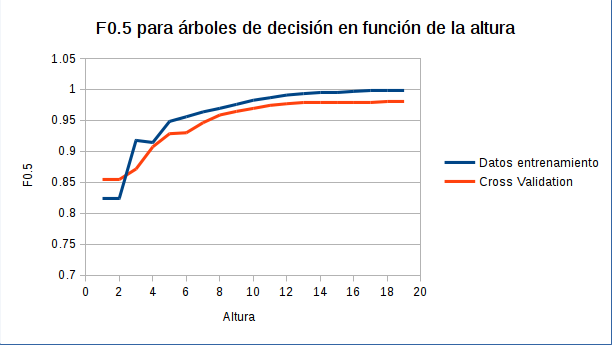
\includegraphics[width=\textwidth]{plots/arboles_f05_en_funcion_altura.png}
        \caption{f0.5 en funcíon de altura de árbol}
        \label{fig:arboles_f05_en_funcion_altura}
\end{figure}

	El resultado de cross validation es un estimador de la eficacia que vamos a obtener clasificando correos nuevos y a pesar de que por lo general no aproxime correctamente la eficacia nos permite predecir que estamos haciendo sobre ajuste de datos de entrenamiento cuando al aumentar la altura baja o se mantiene la eficacia. Como se puede ver en la figura ~\ref{fig:arboles_f05_en_funcion_altura} a partir de arboles de altura 9 el aumento en la eficacia al variar la altura especia a bajar hasta que se estanca llegando a arboles de altura 15. 
    Luego para para este rango de alturas ejecutamos un grid search a fin de obtener los mejores hiper-parametros para el clasificador. 
 \begin{enumerate}
\item \textit{criterio de selección:} Se probaron criterios, gini y ganancia de información. No se observaron grandes diferencias en la eficacia del clasificador al variar el criterio. El mejor resultado se obtuvo con ganancia de información. 
\item \textit{Cantidad máxima de atributos considerados:} Este hiper-parámetro permite limitar la cantidad de atributos considerados al hacer un split.  Tiende a favorecer al aparición de arboles que no sean dominados por los atributos que provean mayor ganancia de información, dado que es posible que varios atributos más débiles trabajando en conjunto logren mejor eficacia.  En las pruebas realizadas se obtuvieron mejores resultados sin limitar la cantidad de atributos
\item \textit{Cantidad mínima de elementos en división:} Limita la división de nodos internos a lo que superen en cantidad de elementos la cantidad especificada. Los mejores resultados se obtuvieron con el valor mínimo de 2. Al aumentar el valor y al mismo tiempo limitar las cantidad de atributos limitados se puede observar una caída de eficacia en cross validation. 
\item \textit{Cantidad mínima de elementos en hojas:} Las hojas del árbol no pueden tener menos de la cantidad especificada. Los mejores resultados se obtuvieron con el valor mínimo de 2. Al igual que con el hiper-parámetro anterior, aumentar el valor y al mismo tiempo limitar las cantidad de atributos limitados se puede observar una caída de eficacia en cross validation.  

\subsection{Random Forest}


La idea de random forest es utlizar múltiples árboles de decisión para mejorar la eficacia del clasificador, reduciendo la alta varianza que se observa en la utilización de un único árbol. Esto es posible gracias al bajo costos que lleva entrenar y consultar a cada árbol. 
 La reducción en la varianza suele ser mas significativa cuando el bosque se arma con árboles que utilicen diferentes atributos. Para lograr esto los atributos utilizados en las divisiones de los nodo al construir el árbol se limitan a un subconjunto aleatorio de los atributos, reduciendo la probabilidad que lo atributos con mayor ganancia de información dominen todos los arboles. 
Utilizando los mismos parámetros que para el clasificador de un único árbol volvimos a hacer pruebas variando la cantidad de árboles del bosque y el tamaño del subconjunto de atributos a considerar. En la figura ~\ref{fig:forest_f05_en_funcion_de_cantidad_de_arboles} se muestran los resultados para bosques de diferentes tamaños considerando n, $\sqrt{n}$ y $\log(n)$ atributos, donde n es la cantidad total de atributos. Los bosques en loas cuales se consideran n atributos muestran mejores resultados, pero cuando consideran $\sqrt{n}$ atributos,  la varianza es inferior por lo que esperamos que la eficacia con datos nuevos sea más parecida a lo  que observamos con cross validation sobre datos de entrenamiento. 

\begin{figure}[H]
\begin{center}
\myss{0.45}{random_forest.pdf}{$f_{0.5}$ en funcíon de cantidad de árboles}{0.35}
\myss{0.45}{random_forest_var.pdf}{varianza enfuncíon de cantidad de árboles}{0.35}
\caption{Resultados grid search random forest}
\label{fig:forest_f05_en_funcion_de_cantidad_de_arboles}
\end{center}
\end{figure}

\subsection{K Vécinos Mas Cercanos}

Para este clasificador consideramos un enfoque parecido al de árbol de decisión, a fin de limitar las pruebas necesarias para conseguir los mejores hiper-parámetros, primero realizamos tests variando la cantidad de vecinos,k, considerados y calculando f0.5 para cross validation de 10 folds. Obteniendo los resultados de la figura ~\ref{fig:knn_f05_en_funcion_vecinos} .
Luego para los valores de k que presentaron mejores resultados ejecutamos un grid search considerando lo siguientes hiper-parámetros. 
\begin{figure}[H]
    \centering
        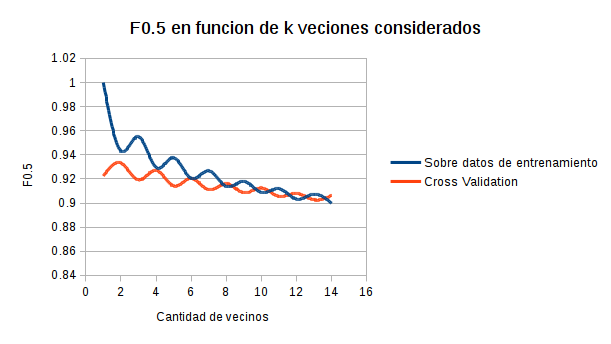
\includegraphics[width=\textwidth]{plots/knn_f05_en_funcion_vecinos.png}
        \caption{f0.5 en funcíon de k vecinos considerados}
        \label{fig:knn_f05_en_funcion_vecinos}
\end{figure}
    Se consideraron los siguiente atributos ademas de la cantidad de vecinos previamente seleccionadas para el grid search:
 \begin{enumerate}
\item \textit{Peso:} Este parámetro ponderar el peso de cada uno de los vecinos por por su distancia o tratarlos a todos uniformemente ignorando la distancia. En nuestro caso se obtuvieron mejores resultados considerando los vecinos uniformemente.  
\item \textit{Métrica de distancia:} Se probaron diferentes métricas de distancias, obteniendo los mejores resultados con la distancia manhattan en la cual la distancia entre dos puntos es la suma de las diferencias absolutas de sus coordenadas.
\end{enumerate}

\subsection{Naive Bayes}

Para este clasificador tuvimos que elegir primero la distribución que asumiriamos que iba a tener $ P(x_i | y) $, las opciones que consideramos fueron una distribución Gaussiana, Binomial y Multinomial. La distribución que mejores resultados obtuvo fue la Binomial lo cual tiene sentido debido a que modela bien la gran cantidad de atributos binarios, quizas si estos tuvieran mas de dos resultados posibles la distribución Multinomial o la Gaussiana habrian sido mejores opciónes.
Los hiperparametros que consideramos fueron $alpha$ y $fit\_prior$ , el primero suaviza la función de distribución de cada atributo y el segundo intenta ir mejorando la estimación de los atributos y las clases a priori, a medida que va analizando nuevas instancias.

\subsection{Support Vector Machine}

Debido a limitaciones de tiempo y computo solo pudimos probar SVM con los parametros dados por defecto en Sklearn, obtuvimos una performance del 83.5\% al realizar cross validation de 10 folds con el set de entrenamiento utilizando F0.5 como medida de score.

SVC(C=1.0, kernel='rbf', degree=3, gamma='auto', coef0=0.0, shrinking=True, probability=False, tol=0.001, cache_size=200, class_weight=None, verbose=False, max_iter=-1, decision_function_shape=None, random_state=None)

\url{http://scikit-learn.org/stable/modules/generated/sklearn.svm.SVC.html#sklearn.svm.SVC}

\end{enumerate}

\newpage

\section{Reducción de dimensionalidad}
Utilizamos distintas técnicas de reduccion de la dimensionalidad PCA, Linear SVC con penalidad L1, ExtraTreesClassifier y simplemente seleccionar los 100 mejores.


\newpage

\section{Resultados en Testing Set}

Luego de experimentar con distintos parametros, clasificadores e hiperparametros terminamos escogiendo -COMPLETAR- con esta versión final de nuestro clasificador de Spam, logramos un f0.5 de -COMPLETAR- sobre el conjunto de testing. 
\newpage

\section{Discusión}
Al  finalizar el trabajo terminamos optando por Random Trees Classier como nuestro algoritmo predilecto, este tuvo la mejor performance, se desempeño bien utilizando los atributos que consideramos y superó en gran medida a los demás clasificadores. La excepción está quizas con Bernoulli Naive Bayes, este metodo también obtuvo resultados muy buenos, al final terminamos descartandolo porque su performance era levemente inferior pero quedaron en el tintero varias ideas que quedarán como trabajo a futuro, consideramos crear un clasicador que corra ambos metodos (Random Trees y Naive Bayes) y decida como un arbitro a cual hacerle caso o que conteste con cierto nivel de seguridad segun si ambos responden igual o no. Otro tema a explotar podría ser el del preprocesamiento, la falencia del mismo nos trajo problemas al buscar palabras clave en los textos ya que el código html generaba ruido en los resultados, de todas maneras pudimos superar dichos problemas parcialmente y conseguimos un corpus de palabras que creemos se desempeña de forma bastante exitosa.
\newpage
% the \\ insures the section title is centered below the phrase: AppendixA

\end{document}
